\documentclass[man]{apa7}

\input{includes/preamble_common}
\input{includes/preamble_apa7}

\title{Integración de Patrones de Diseño (MVC) y Frameworks (Spring Boot vs Node.js) en el Desarrollo Backend de Aplicaciones Web}
\shorttitle{Integración de Patrones de Diseño}
\authorsnames{Cristofer David Lozano Contreras}
\authorsaffiliations{Análisis y Desarrollo de Software, SENA}
\authornote{Instructor: Jesús Ariel González Bonilla. Fecha: 28 de septiembre de 2025}

\abstract{El objetivo de este artículo es analizar la integración de frameworks backend y patrones de diseño, específicamente el Modelo-Vista-Controlador (MVC), en el desarrollo de servicios web. Se destaca la importancia de los servicios RESTful en la comunicación entre cliente y servidor, como una alternativa eficiente a tecnologías legadas, utilizando métodos HTTP (GET, POST, PUT, DELETE). El estudio se centra en la comparación de dos frameworks principales: Spring Boot (Java) y Node.js (JavaScript), reconociendo sus fortalezas distintivas: Spring Boot por su robustez, seguridad y orientación empresarial, y Node.js por su rapidez, asincronía y escalabilidad en aplicaciones que requieren baja latencia. La integración del patrón MVC es crucial para la organización, mantenibilidad y testabilidad del código, ya que separa la lógica de negocio (Modelo), la interfaz (Vista) y el flujo de control (Controlador). Se concluye que la elección del framework backend (Spring Boot o Node.js) debe estar alineada con el contexto del proyecto, las necesidades de seguridad y la madurez del equipo, demostrando que la combinación de arquitecturas sólidas y herramientas adecuadas, gestionadas bajo la Metodología Scrum, es fundamental para el éxito del software.
}

\keywords{Servicios RESTful, Spring Boot, Node.js, Patrones de diseño, Modelo Vista Controlador, Backend}

\begin{document}
\maketitle

\section{Introducción}
El desarrollo de software contemporáneo enfrenta retos significativos, derivados de la necesidad de construir sistemas escalables, seguros y mantenibles. En el ámbito del desarrollo backend, la comunicación eficiente entre el cliente y el servidor se ha convertido en un pilar, popularizando los servicios Web RESTful por su simplicidad y eficiencia frente a tecnologías más complejas como SOAP.
Para abordar la creciente complejidad del código y asegurar su calidad a largo plazo, la comunidad técnica ha promovido la adopción de estructuras de diseño y paradigmas que fomentan la separación de responsabilidades y la reutilización. En este sentido, la elección del framework backend es vital, donde Spring Boot y Node.js se presentan como contendientes robustos. De forma complementaria, la aplicación de patrones arquitectónicos como el Modelo-Vista-Controlador (MVC) busca imponer modularidad, coherencia y claridad, facilitando las pruebas unitarias y la evolución del sistema.
En este contexto, el presente trabajo busca analizar y aplicar estas prácticas a nivel técnico, con el objetivo de demostrar que la integración de frameworks backend maduros (como Spring Boot y su afinidad con MVC) junto con la aplicación de la metodología Scrum, favorece la creación de sistemas más robustos, seguros y alineados con los requisitos funcionales del proyecto.
\section{Marco teórico y trabajos relacionados}
\subsection{Patrón de diseño}
Los patrones de diseño constituyen soluciones ya probadas y estructuradas para problemas recurrentes en el desarrollo de software. Su objetivo principal es evitar la duplicación de código y favorecer su reutilización, aportando claridad y modularidad en los sistemas \cite{gavilanez2022analisis}. En el desarrollo backend, patrones como el Modelo-Vista-Controlador (MVC) son cruciales para mantener una lógica de organización que facilita el mantenimiento y la comprensión por parte de otros desarrolladores \cite{zambrano_patron}.

\subsection{Arquitectura de software y seguridad}
La arquitectura de software se concibe como la estructura fundamental de un sistema, que facilita la escalabilidad, el mantenimiento y la comprensión global del sistema. En el contexto backend, una arquitectura bien definida es indispensable, ya que la seguridad del software está estrechamente vinculada a la calidad de su desarrollo. La falta de organización y metodologías claras no solo dificulta la evolución del software, sino que también incrementa los riesgos y vulnerabilidades en sistemas críticos.

\subsection{Modelo-Vista-Controlador (MVC)}
El patrón Modelo-Vista-Controlador (MVC) organiza una aplicación en tres componentes principales con el propósito de reducir el acoplamiento y estandarizar el diseño:
•	Modelo: Encargado de la gestión de datos, reglas de negocio y estado.
•	Vista: Define la interfaz de usuario y muestra la información al usuario.
•	Controlador: Actúa como intermediario, gestionando las interacciones y solicitudes del usuario para actualizar el Modelo o la Vista.
Esta separación favorece la mantenibilidad y la testabilidad del software, permitiendo trabajar de forma independiente en cada componente \cite{hernandez2015guia}. En el desarrollo backend, el MVC es vital para la organización de los servicios REST, donde el Controlador gestiona las peticiones y el Modelo maneja la lógica de negocio y la persistencia de datos.

\subsection{Servicios Web RESTful (Backend)}
Los servicios REST (Representational State Transfer) son un estilo arquitectónico que se apoya en el protocolo HTTP para la comunicación entre cliente y servidor. Se han convertido en la base del desarrollo backend moderno debido a su simplicidad, facilidad de implementación y escalabilidad frente a tecnologías como SOAP y WSDL. Utilizan métodos HTTP estándar (GET, POST, PUT, DELETE) para realizar operaciones CRUD (Crear, Leer, Actualizar, Borrar) sobre recursos.

\subsection{Frameworks Backend: Spring Boot vs Node.js}
La elección del framework backend es determinante para el éxito del proyecto \cite{haro2019nodejs}.

No existe un framework superior, sino que la elección debe responder al contexto del proyecto, las necesidades de seguridad y la experiencia del equipo \cite{brito_consideraciones}.
\section{Metodología de investigación aplicada}
El presente proyecto se desarrolló bajo un enfoque cualitativo, orientado a la comprensión e interpretación de conceptos relacionados con el patrón Modelo-Vista-Controlador (MVC), la arquitectura de Servicios Web RESTful y la comparación de frameworks backend como Spring Boot y Node.js. La implementación práctica se gestionó bajo la metodología ágil Scrum.

\subsection{Fase 1: Recolección y construcción del thesaurus}
Se utilizó Google Scholar, realizando consultas con palabras clave como: MVC, Servicios RESTful, Spring Boot, Node.js, Seguridad en aplicaciones web. El propósito fue reunir evidencia científica que respaldara el uso del patrón MVC, la arquitectura REST y la idoneidad de los frameworks backend seleccionados para la construcción de sistemas robustos y seguros.

\subsection{Fase 2: Análisis cualitativo de la evidencia (síntesis del thesaurus)}
El objetivo fue transformar la información documental en argumentos sólidos que justificaran la elección de MVC y el análisis comparativo entre Spring Boot y Node.js.
•	Se realizó una lectura crítica para identificar las ventajas del MVC en términos de separación de responsabilidades, mantenibilidad y testabilidad.
•	Se analizaron las características clave de Spring Boot y Node.js para determinar su aplicabilidad en diferentes contextos de proyecto.
•	Se consideraron las vulnerabilidades y riesgos comunes en aplicaciones web (como inyección SQL o XSS) para enfocar la implementación en la seguridad del backend.

\subsection{Fase 3: Diseño y desarrollo del sistema}
Transformar los criterios teóricos y metodológicos en un sistema funcional de servicios web, aplicando la arquitectura MVC y Servicios RESTful como guías de construcción y organización del proyecto.

\subsubsection{Procedimiento detallado}
\paragraph{1. Diseño de la Arquitectura (MVC con REST):}
o	Se definieron las capas principales: Modelo (lógica de negocio y persistencia de datos), y Controlador (gestión de las peticiones REST, mapeando verbos HTTP a operaciones del Modelo).
o	Esta separación permite mejorar la mantenibilidad y la escalabilidad del backend.

\paragraph{2. Selección y aplicación de Frameworks (Spring Boot como base):}
o	Se priorizó Spring Boot (Java) para la implementación base de los servicios RESTful, debido a su robustez y alto nivel de seguridad, ideal para un entorno formativo que simula exigencias empresariales.
o	Se utilizó el patrón Programación Orientada a Objetos (POO) en Java para estructurar el código bajo principios de herencia, encapsulamiento y polimorfismo, garantizando un desarrollo ordenado y reutilizable.

\paragraph{3. Metodología Ágil (Scrum):}
o	Se implementó la metodología Scrum, realizando reuniones clave (como la Daily Scrum) y trabajando por sprints definidos, lo que permitió ajustar prioridades y detectar errores de manera temprana.

\subsubsection{Herramientas utilizadas}
•	Backend: Java con Spring Boot (por su robustez y seguridad).
•	Base de datos: PostgreSQL (para gestionar la información de recursos).
•	Herramientas de Desarrollo: Visual Studio Code (VSC) (IDE ligero y flexible).
•	Gestión de Dependencias: Maven (para la gestión de librerías y ciclo de vida de proyectos Java).
•	Control de versiones: GitHub (para trabajo colaborativo y control de cambios).
\section{Implementación del software}
\subsection{C. Fase 3- Diseño y desarrollo del sistema}
Transformar los criterios teóricos y metodológicos en un sistema funcional de gestión de eventos, aplicando la arquitectura MVC, la POO y la metodología ágil Scrum como guías de construcción y organización del proyecto.

\subsubsection{Procedimiento detallado}
\paragraph{1. Diseño de la arquitectura (MVC):}
• Se definieron las capas principales del sistema: Modelo (gestión de datos y lógica de negocio), Vista (interfaces gráficas de usuario) y Controlador (coordinación de entradas/salidas y flujo de información).

• Esta separación permitió mejorar la mantenibilidad y la escalabilidad del sistema, ya que cada capa pudo evolucionar de manera independiente.

\paragraph{2. Programación Orientada a Objetos (POO):}
• Se estructuró el código bajo principios de herencia, encapsulamiento y polimorfismo, lo cual garantizó un desarrollo más ordenado y reutilizable.

• El uso de POO facilitó la construcción de módulos comunes para diferentes funcionalidades, como gestión de usuarios, administración de eventos y reportes.

\paragraph{3. Metodología Ágil Scrum:}
• Se realizaron reuniones periódicas de seguimiento y retroalimentación, permitiendo ajustar prioridades y detectar errores de manera temprana.

\paragraph{4. Herramientas utilizadas:}
• Backend: Java con Spring Boot, seleccionado por su robustez, seguridad y escalabilidad.

• Frontend web: React.js, elegido por su flexibilidad en el diseño de interfaces dinámicas.

• Aplicación móvil: React Native, lo que permitió extender las funcionalidades al entorno móvil sin duplicar esfuerzos de programación.

• Base de datos: PostgreSQL, empleada para gestionar la información de usuarios, eventos y reservas.

• Control de versiones: GitHub, para trabajo colaborativo y control de cambios en el código.
\section{Evaluación y resultados}
Se concluyó que el desarrollo de un sistema backend requiere de una arquitectura sólida (MVC) sustentada en un paradigma adecuado (POO), lo que garantiza la organización del software y su seguridad. Asimismo, la importancia de emplear una metodología debidamente estructurada (Scrum) permite adaptarse a los cambios y mejorar la comunicación.
Estos hallazgos no solo orientaron la decisión técnica hacia Spring Boot para el entorno empresarial, sino que también aportaron criterios prácticos para optimizar la colaboración del equipo y la calidad del producto desarrollado.

\subsection{Resultados en la arquitectura y el desarrollo del sistema Backend}
Se obtuvo un backend basado en la arquitectura Modelo-Vista-Controlador (MVC), implementado con Servicios RESTful que permiten:
Separación de Responsabilidades: El Controlador gestiona las peticiones HTTP y el Modelo maneja la lógica de negocio y la conexión a PostgreSQL.
Reutilización y Escalabilidad: La adopción de la Programación Orientada a Objetos (POO) con Spring Boot aportó principios como la reutilización y el encapsulamiento, garantizando un desarrollo más estructurado y con mayor facilidad para la mantenibilidad y evolución futura del sistema.
Seguridad Mejorada: La madurez de Spring Boot facilita la implementación de características de seguridad críticas, abordando vulnerabilidades comunes en aplicaciones web.

\begin{figure}[htbp]
    \centering
    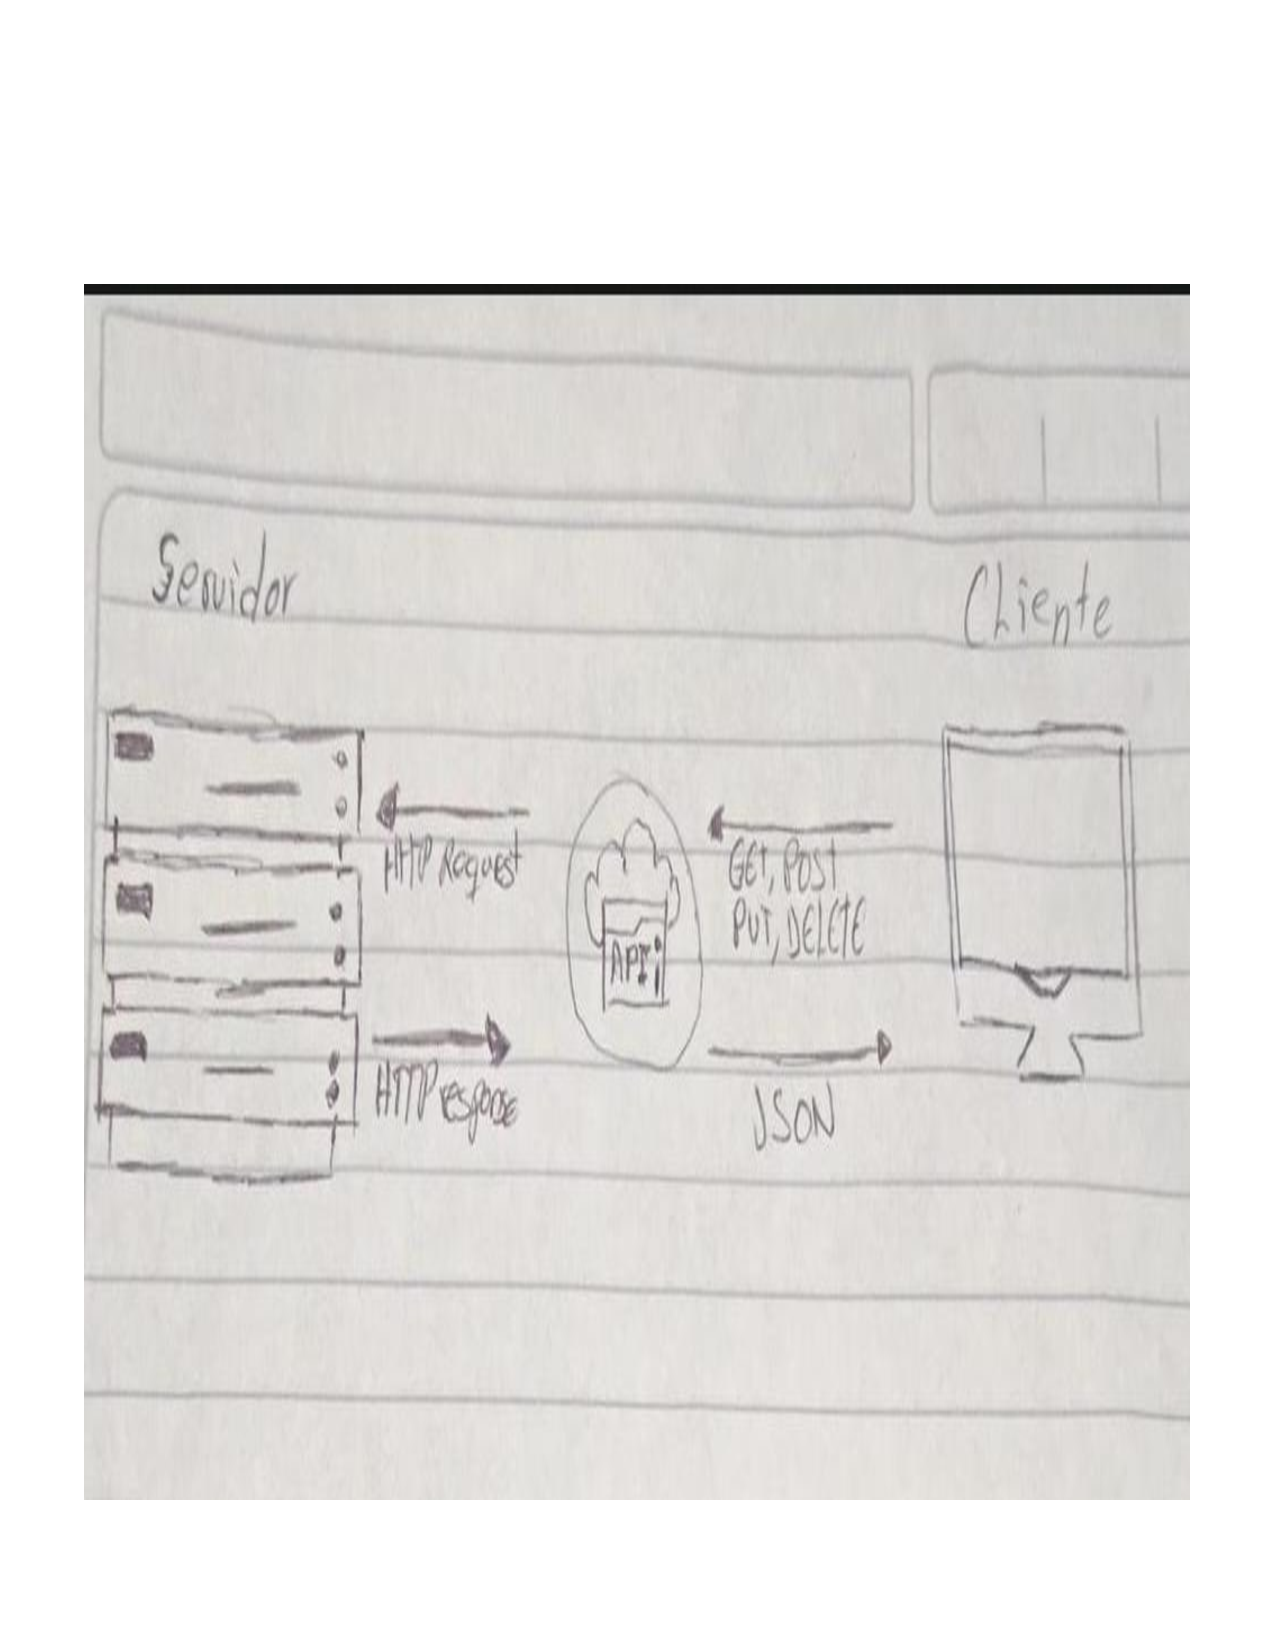
\includegraphics[width=0.48\textwidth]{graphics/SERVICIOS.pdf}
    \caption{Arquitectura de Servicios RESTful}
    \label{fig:servicios}
\end{figure}

En la Figura \ref{fig:servicios} se ilustra la arquitectura de comunicación de los servicios. Esta muestra cómo el API RESTful funciona como la capa central que media la transferencia de datos entre los servidores backend (donde reside la lógica) y la aplicación cliente. Este enfoque de servicios permitió la total desconexión del backend del frontend, facilitando la escalabilidad del sistema \cite{hernandez2015guia}.

\subsection{Resultados en la aplicación de la metodología ágil (Scrum)}
La implementación de la metodología ágil Scrum generó beneficios en la organización y el seguimiento del trabajo backend:
•	Planificación y Control: La organización en sprints y el uso de un tablero Kanban (e.g., Trello) permitieron la visualización clara de las tareas (diseño del API, implementación del Controlador, lógica del Modelo, pruebas).
•	Comunicación: Las reuniones de seguimiento fomentaron la comunicación constante y la responsabilidad compartida, esenciales para la resolución de bugs y la adaptación a cambios de requisitos.

\begin{figure}[htbp]
    \centering
    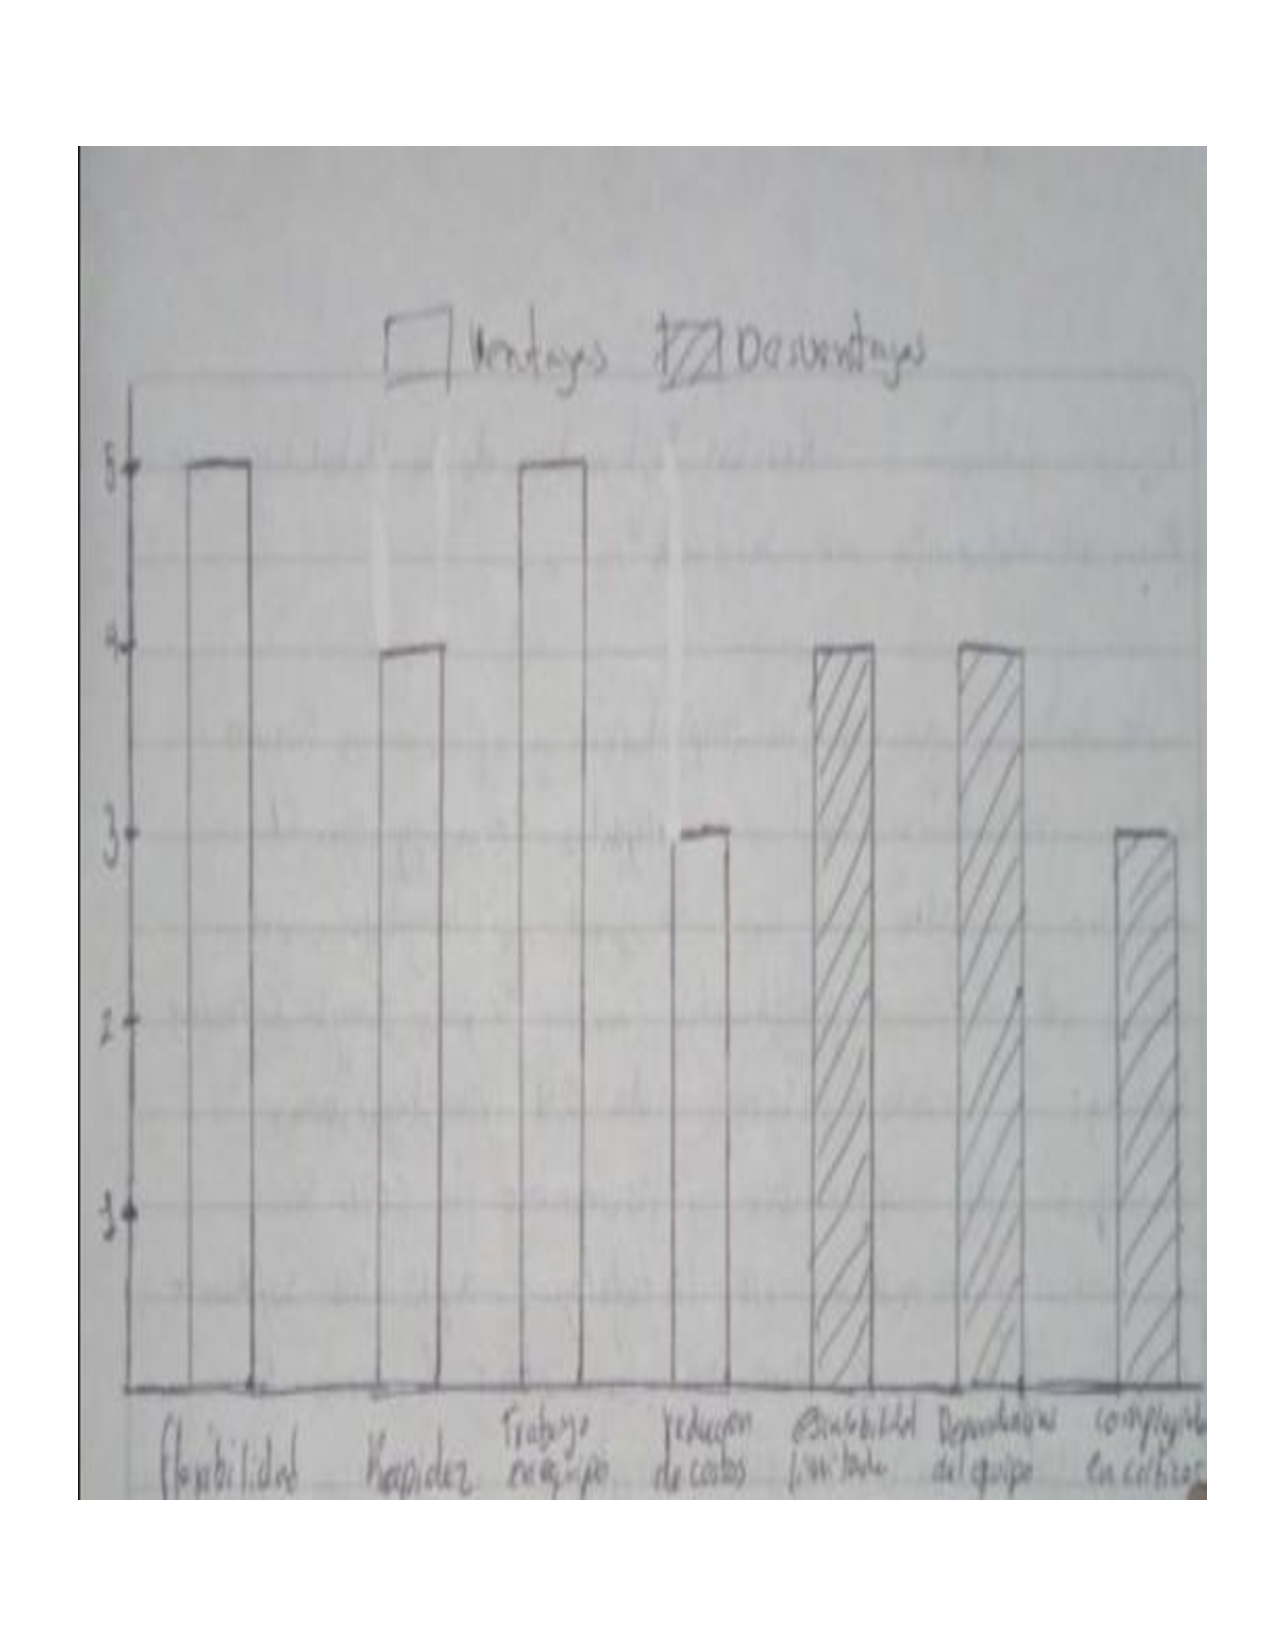
\includegraphics[width=0.48\textwidth]{graphics/DiagramaScrum.pdf}
    \caption{Diagrama de los beneficios de Scrum}
    \label{fig:scrum}
\end{figure}

En la Figura \ref{fig:scrum} se observa el diagrama de los beneficios de Scrum, que ilustra cómo esta metodología ágil mejora la planificación, control y comunicación en el desarrollo de proyectos backend \cite{brito_consideraciones}.

\input{sections/06_discusion}
\section{Conclusiones y trabajo futuro}
A partir de la metodología cualitativa implementada, se evidenció que la combinación de una arquitectura sólida (MVC/REST) y una metodología ágil (Scrum) resulta fundamental para el éxito en el desarrollo de sistemas.
La revisión documental comparativa entre Spring Boot y Node.js confirmó que no existe un framework superior, sino que la elección se basa en la correcta alineación entre la tecnología seleccionada, los objetivos del proyecto y las competencias del equipo:
•	Spring Boot: Ideal para proyectos que requieren solidez, alta seguridad y madurez (entornos empresariales).
•	Node.js: Mejor opción para aplicaciones que necesitan flexibilidad, rapidez y alta escalabilidad con tiempos de respuesta cortos.
La aplicación del patrón MVC facilita la organización, escalabilidad y mantenibilidad del código, mientras que el uso de Scrum fortaleció la planificación y la entrega incremental de funcionalidades. Estos hallazgos validan que la investigación teórica y la práctica de desarrollo backend deben estar alineadas para lograr un producto funcional y sustentable a largo plazo.
\appendix
% Apéndices adicionales si es necesario

\printbibliography

\end{document}